%! Author = Wiktor Rostkowski, Mateusz Budzisz
%! Date = 05/1/2024

\chapter{Opis problemu}
\label{ch:opis-problemu}

\section{Przestawienie problemu}
\label{sec:przestawienie-problemu}

Analizując swoje potrzeby jako turystów, zespół projektowy zauważył liczne obszary,~w~których aplikacja może znacząco wspierać turystów.
W trakcie~tej~analizy, członkowie zespołu zidentyfikowali konkretne wyzwania~i~problemy,~z~jakimi turyści często~się~borykają.

Pierwszą kwestią jest natłok informacji, który może przytłoczyć turystów.
Podczas poszukiwania informacji~o~atrakcjach turystycznych, turyści~są~bombardowani ogromną ilością niepotrzebnych danych, takich~jak~punkty zainteresowań, które~w~rzeczywistości~nie~są atrakcjami turystycznymi.
Na przykład, korzystając~z~map Google, Bing~lub~Apple, użytkownicy często otrzymują wyniki, które oprócz rzeczywistych atrakcji turystycznych, zawierają również miejsca niezwiązane~z~turystyką, takie~jak~stacje benzynowe, szpitale~i~inne obiekty użyteczności publicznej.
Taka sytuacja utrudnia szybkie~i~efektywne znalezienie informacji~o~faktycznych atrakcjach, powodując frustrację~i~dezorientację użytkowników.
Dlatego niezwykle ważne jest,~aby~aplikacja skierowana~do~turystów była~w~stanie filtrować~i~precyzyjnie dostarczać informacje, które~są~istotne~i~wartościowe~z~punktu widzenia osób podróżujących.

Kolejnym problematycznym obszarem jest dostęp~do~godzin otwarcia~i~aktualność tych danych, które często~są~powielone~w~różnych wersjach~w~wielu miejscach.
Turystom zdarza~się~spotkać~z~rozbieżnościami~w~informacjach~na~temat godzin otwarcia muzeów, parków, restauracji~i~innych atrakcji turystycznych.
Na przykład, godziny otwarcia podane~na~oficjalnej stronie internetowej mogą różnić~się~od tych zamieszczonych~na~platformach społecznościowych, portalach recenzji~lub~w przewodnikach turystycznych.
Takie niespójności mogą prowadzić~do~nieporozumień~i~frustracji, kiedy turyści pojawiają~się~w miejscu, które miało~być~otwarte,~ale~okazuje~się~zamknięte.
Dlatego ważne jest,~aby~aplikacja~dla~turystów mogła zapewniać zaktualizowane, spójne~i~wiarygodne informacje~o~godzinach otwarcia, minimalizując ryzyko takich problemów~i~ułatwiając planowanie zwiedzania.

Trzecim~z~problematycznych obszarów jest skomplikowanie rozłożenia zwiedzania~na~poszczególne dni.
Ręczne tworzenie takiego planu wymaga zaawansowanych zdolności analitycznych oraz dużego nakładu pracy,~a~mimo~to~jest bardzo podatne~na~błędy.
Tworzony~w~ten sposób plan często szybko~się~dezaktualizuje,~co~wymusza konieczność jego ponownego przemyślenia~i~wykonania~od~nowa.
Chociaż istnieją narzędzia wspomagające planowanie dnia, konieczność ręcznego wprowadzania godzin otwarcia atrakcji turystycznych sprawia,~że~ich użycie może~być~bardziej czasochłonne~niż~przynoszące korzyści.
W efekcie, zamiast ułatwiać planowanie, narzędzia~te~często komplikują proces, zniechęcając użytkowników~do~ich stosowania.
Aby rzeczywiście wspomóc turystów~w~efektywnym planowaniu, aplikacja powinna automatycznie integrować aktualne informacje~o~godzinach otwarcia, dostarczając kompleksowe~i~łatwe~w~użyciu narzędzie~do~tworzenia planów zwiedzania.
Dzięki temu turyści będą mogli skupić~się~na cieszeniu~się~podróżą,~a~nie~na~logistyce~jej~organizacji.

Ostatnim obszarem wymagającym usprawnień jest ułożenie trasy~z~wykorzystaniem komunikacji miejskiej pomiędzy wieloma punktami.
Gdy użytkownik stworzy plan zwiedzania, powinien mieć automatyczną możliwość zobaczenia dostępnych połączeń między wybranymi atrakcjami~bez~konieczności ręcznego wyszukiwania informacji~o~dostępnych środkach transportu.
Wprowadzenie takiej funkcji~w~aplikacji turystycznej znacznie ułatwiłoby podróżowanie, eliminując potrzebę czasochłonnego~i~często skomplikowanego poszukiwania informacji~o~trasach, rozkładach jazdy~i~przesiadkach.
Automatyczna integracja danych~o~komunikacji miejskiej zapewniłaby turystom łatwy dostęp~do~aktualnych~i~precyzyjnych informacji,~co~przyczyniłoby~się~do bardziej efektywnego planowania czasu oraz zwiększenia komfortu podróżowania.
Dzięki temu turyści mogliby skupić~się~na zwiedzaniu~i~czerpaniu przyjemności~z~odkrywania nowych miejsc, mając pewność,~że~aplikacja zadba~o~logistyczne aspekty~ich~podróży.

\pagebreak
\section{Rich picture}
\label{sec:rich-picture}

Rich picture, czyli wzbogacony wizerunek, jest graficznym przedstawieniem problemu, które ilustruje różnorodne aspekty~i~zależności związane~z~danym zagadnieniem.
Poniżej znajduje~się~graficzne ujęcie problemów napotykanych przez turystów~\ref{fig:rich-picture}.

\begin{figure}[h]
    \centering
    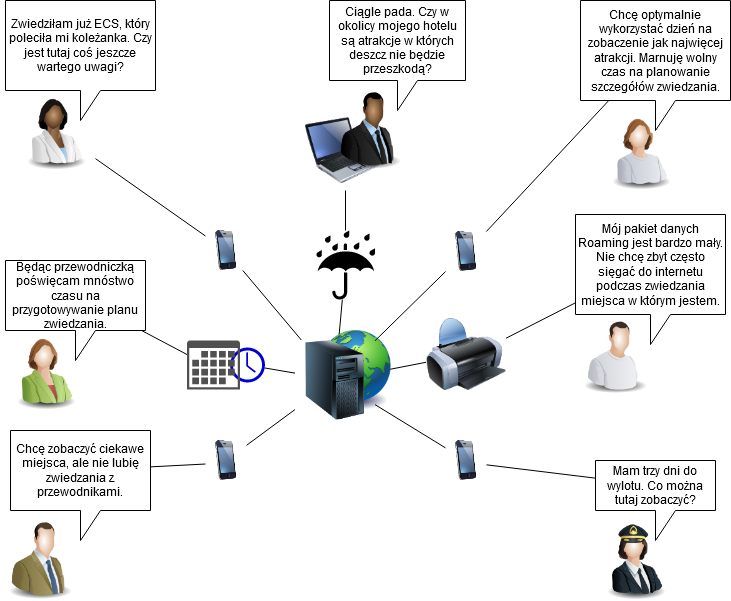
\includegraphics[width=1\textwidth]{attachments/rich-picture}
    \caption{Wzbogacony wizerunek planeru miejskiego}
    \label{fig:rich-picture}
\end{figure}

\pagebreak
\section{Cele projektu}
\label{sec:cele-projektu}

TODO
